\documentclass[a4paper,12pt]{article}
\usepackage[utf8]{inputenc}
\usepackage{amsmath}
\usepackage{amssymb}
\usepackage{amsthm}
\usepackage{geometry}
\usepackage{graphicx}
\usepackage[hidelinks]{hyperref}
\usepackage{listings}
\usepackage{xcolor}
\usepackage{enumitem}
\usepackage{booktabs}
\usepackage{array}
\usepackage{float}

\geometry{margin=2.5cm}

\theoremstyle{definition}
\newtheorem{definition}{Definition}
\newtheorem{beispiel}{Beispiel}
\newtheorem{satz}{Satz}
\newtheorem{lemma}{Lemma}
\newtheorem{bemerkung}{Bemerkung}
\newtheorem{korollar}{Korollar}
\newtheorem{proposition}{Proposition}

\setlist[itemize,1]{label=--}

% ---------- Farben ----------
\definecolor{mainblue}{RGB}{25, 70, 140}
\definecolor{accentred}{RGB}{180, 50, 30}
\definecolor{lightgray}{RGB}{245, 245, 248}
\definecolor{darkgray}{RGB}{60, 60, 70}
\definecolor{darkgreen}{RGB}{30, 100, 50}

\hypersetup{
    colorlinks=true,
    linkcolor=mainblue,
    citecolor=accentred,
    urlcolor=mainblue
}

% Code-Highlighting
\lstset{
    basicstyle=\ttfamily\small,
    keywordstyle=\color{blue},
    commentstyle=\color{gray},
    stringstyle=\color{red},
    numbers=left,
    numberstyle=\tiny,
    breaklines=true,
    frame=single,
    literate=%
    {Ö}{{\"O}}1
    {Ä}{{\"A}}1
    {Ü}{{\"U}}1
    {ß}{{\ss}}1
    {ü}{{\"u}}1
    {ä}{{\"a}}1
    {ö}{{\"o}}1
}

\title{Der Dirac-Impuls: Formale Theorie, Eigenschaften und Anwendungen\\[0.5em]
\large Eine umfassende Darstellung im Rahmen der Distributionentheorie}
\author{Stephan Epp\\
Universit\"at Bielefeld}
\date{3. Juni 2026}

\begin{document}

\maketitle

\begin{abstract}
Der Dirac-Impuls $\delta(t)$ -- auch Dirac-Delta-Distribution oder Einheitsimpuls genannt -- nimmt
in der mathematischen Analysis, der Funktionalanalysis und insbesondere in der Signal- und
Systemtheorie eine herausragende Stellung ein. Obwohl er keiner klassischen Funktion entspricht
und formal als verallgemeinerte Funktion (Distribution) aufzufassen ist, hat sich um ihn ein
vollst\"andiger, strenger mathematischer Rahmen entwickelt, der auf der Distributionentheorie von
Laurent Schwartz beruht. Die zentrale Eigenschaft des Dirac-Impulses ist, dass er bei $t=0$
\emph{konzeptionell unendlich hoch} ist, aber seine Fl\"ache stets exakt gleich~$1$ bleibt.
Diese scheinbar paradoxe Eigenschaft wird in der vorliegenden Arbeit rigoros hergeleitet, formal
bewiesen und durch numerische Approximationen sowie Visualisierungen gest\"utzt. Zus\"atzlich
werden alle wesentlichen Eigenschaften -- Siebungseigenschaft, Fourier-Darstellung, Faltungsidentit\"at,
Skalierungsinvarianz und Zusammenhang zur Heaviside-Funktion -- vollst\"andig bewiesen. Ein
ausf\"uhrlicher Ausblick beleuchtet offene Forschungsrichtungen und Anwendungsgebiete.
\end{abstract}

\tableofcontents
\newpage

% =====================================================================
\section{Einf\"uhrung}
% =====================================================================

Der Begriff des \emph{Dirac-Impulses} geht auf den britischen Physiker Paul Adrien Maurice Dirac
zur\"uck, der diese Konstruktion 1927 in der Quantenmechanik einsetzte \cite{dirac1927}. Dirac
ben\"otigte ein Objekt, das formal wie eine Funktion behandelt werden kann, aber die Eigenschaft
hat, an einem einzigen Punkt den gesamten Wert $1$ zu konzentrieren. Er schrieb:
\begin{quote}
``$\delta(x) = 0$ for $x \neq 0$, and $\int_{-\infty}^{\infty} \delta(x)\,dx = 1$.''
\end{quote}
Aus klassisch-mathematischer Sicht ist dies widerspr\"uchlich: Eine Funktion, die \"uberall
au{\ss}er an einem einzigen Punkt $0$ ist, hat nach dem Lebesgue-Integral den Integralwert $0$,
nicht $1$. Dieses Dilemma wurde erst 1945--1950 durch Laurent Schwartz mit seiner
\emph{Distributionentheorie} \cite{schwartz1950} vollst\"andig aufgel\"ost.

\subsection{Problemstellung und Motivation}

In Natur und Technik begegnet man h\"aufig Vorg\"angen, die auf einer sehr kurzen Zeitskala
eine gro{\ss}e Wirkung entfalten: Ein Hammerschlag auf ein Werkst\"uck, ein Blitzschlag, der
Startimpuls eines Digitalschaltkreises oder die Messung eines Neutrinos. Diese Ph\"anomene
lassen sich mathematisch am naturgem\"a{\ss}esten durch den Dirac-Impuls modellieren.

\textbf{Zentrales Paradoxon:} Der Dirac-Impuls $\delta(t)$ ist:
\begin{itemize}
    \item unendlich hoch bei $t = 0$,
    \item gleich $0$ f\"ur alle $t \neq 0$,
    \item hat aber dennoch eine Fl\"ache von exakt $1$ unter sich.
\end{itemize}
Die vorliegende Arbeit zeigt, dass dieses ``Paradoxon'' durch den Grenzwert-Charakter von
$\delta$ als distributionellen Grenzobjekt vollst\"andig aufgel\"ost wird.

\subsection{Struktur der Arbeit}

Abschnitt~\ref{sec:grundlagen} legt die mathematischen Grundlagen der Distributionentheorie.
Abschnitt~\ref{sec:definition} definiert den Dirac-Impuls rigoros und beweist die
Normierungseigenschaft. Abschnitt~\ref{sec:eigenschaften} leitet alle wesentlichen Eigenschaften
formal her. Abschnitt~\ref{sec:naherungen} behandelt die Approximationsfolgen mit Visualisierungen.
Abschnitt~\ref{sec:lti} zeigt Anwendungen in Signal-, System- und Quantentheorie.
Abschnitt~\ref{sec:ausblick} enth\"alt einen ausf\"uhrlichen Forschungsausblick.

% =====================================================================
\section{Mathematische Grundlagen}
\label{sec:grundlagen}
% =====================================================================

\subsection{Testfunktionen und der Schwartz-Raum}

\begin{definition}[Testfunktionenraum $\mathcal{D}(\mathbb{R})$]
\label{def:testfunktionen}
Sei $\mathcal{D}(\mathbb{R})$ die Menge aller glatten Funktionen mit kompaktem Tr\"ager:
\[
\mathcal{D}(\mathbb{R}) \;:=\;
\bigl\{\,\varphi \in C^\infty(\mathbb{R}) \;\big|\;
\operatorname{supp}(\varphi) \text{ ist kompakt}\bigr\}.
\]
Diese Menge wird versehen mit einer geeigneten Topologie, die durch Seminormen definiert ist.
\end{definition}

\begin{beispiel}
Die Funktion
\[
\varphi(t) = \begin{cases}
\exp\!\left(\dfrac{-1}{1-t^2}\right) & |t| < 1 \\
0 & |t| \geq 1
\end{cases}
\]
liegt in $\mathcal{D}(\mathbb{R})$ und ist ein prototypisches Beispiel einer Testfunktion.
\end{beispiel}

\begin{definition}[Schwartz-Raum $\mathcal{S}(\mathbb{R})$]
Der \emph{Schwartz-Raum} ist definiert als
\[
\mathcal{S}(\mathbb{R}) := \bigl\{\, f \in C^\infty(\mathbb{R}) \;\big|\;
\forall \alpha, \beta \in \mathbb{N}_0:\; \sup_{t \in \mathbb{R}} |t^\alpha f^{(\beta)}(t)| < \infty \bigr\},
\]
d.\,h.\ die Menge aller glatten Funktionen, deren Ableitungen schneller als jede Potenz abfallen.
\end{definition}

\begin{definition}[Distribution]
\label{def:distribution}
Eine \emph{Distribution} (oder \emph{verallgemeinerte Funktion}) ist ein stetiges lineares Funktional
$T: \mathcal{D}(\mathbb{R}) \to \mathbb{R}$. Die Menge aller Distributionen wird mit
$\mathcal{D}'(\mathbb{R})$ bezeichnet.
\end{definition}

\begin{bemerkung}
Jede lokal integrierbare Funktion $f \in L^1_{\mathrm{loc}}(\mathbb{R})$ definiert durch
\[
T_f[\varphi] := \int_{-\infty}^{\infty} f(t)\,\varphi(t)\,dt
\]
eine Distribution. Umgekehrt gibt es Distributionen, die keine regularen Funktionen sind --
der Dirac-Impuls ist das prominenteste Beispiel.
\end{bemerkung}

\subsection{Konvergenz im Distributionensinne}

\begin{definition}[Schwache Konvergenz]
Eine Folge $(T_n)$ in $\mathcal{D}'(\mathbb{R})$ \emph{konvergiert schwach} gegen $T \in \mathcal{D}'(\mathbb{R})$,
wenn f\"ur alle $\varphi \in \mathcal{D}(\mathbb{R})$ gilt:
\[
\lim_{n \to \infty} T_n[\varphi] = T[\varphi].
\]
\end{definition}

% =====================================================================
\section{Definition und Normierung des Dirac-Impulses}
\label{sec:definition}
% =====================================================================

\subsection{Formale Definition}

\begin{definition}[Dirac-Impuls]
\label{def:dirac}
Der \emph{Dirac-Impuls} $\delta \in \mathcal{D}'(\mathbb{R})$ ist das lineare Funktional:
\[
\delta[\varphi] := \varphi(0)
\qquad \forall\, \varphi \in \mathcal{D}(\mathbb{R}).
\]
Allgemeiner ist der verschobene Dirac-Impuls $\delta_{t_0}$ definiert durch:
\[
\delta_{t_0}[\varphi] = \delta(t - t_0)[\varphi] := \varphi(t_0).
\]
\end{definition}

\begin{satz}[Wohldefiniertheit und Stetigkeit]
\label{satz:stetigkeit}
$\delta$ ist eine wohldefinierte Distribution, d.\,h.\ $\delta \in \mathcal{D}'(\mathbb{R})$.
\end{satz}

\begin{proof}
Wir m\"ussen zeigen, dass $\delta$ linear und stetig ist.

\textbf{Linearit\"at:} F\"ur $\varphi, \psi \in \mathcal{D}(\mathbb{R})$ und $\lambda \in \mathbb{R}$:
\[
\delta[\lambda\varphi + \psi] = (\lambda\varphi + \psi)(0) = \lambda\varphi(0) + \psi(0)
= \lambda\,\delta[\varphi] + \delta[\psi]. \quad \checkmark
\]

\textbf{Stetigkeit:} Es ist zu zeigen, dass aus $\varphi_n \to 0$ in $\mathcal{D}(\mathbb{R})$
auch $\delta[\varphi_n] \to 0$ folgt. Konvergenz in $\mathcal{D}(\mathbb{R})$ bedeutet insbesondere
gleichm\"a{\ss}ige Konvergenz, also $\sup_t |\varphi_n(t)| \to 0$. Daher:
\[
|\delta[\varphi_n]| = |\varphi_n(0)| \;\leq\; \sup_{t \in \mathbb{R}} |\varphi_n(t)| \;\to 0. \quad \checkmark
\]
\end{proof}

\subsection{Die Normierungseigenschaft: Fl\"ache ist stets 1}

Dies ist die zentrale Eigenschaft des Dirac-Impulses, die in der Physik und Ingenieurwissenschaft
die Aussage ``unendlich hoch, aber Fl\"ache gleich 1'' formalisiert.

\begin{satz}[Normierungseigenschaft]
\label{satz:normierung}
Im Sinne der Distributionentheorie gilt:
\[
\int_{-\infty}^{\infty} \delta(t)\,dt = 1.
\]
\end{satz}

\begin{proof}
Der Ausdruck $\int_{-\infty}^{\infty} \delta(t)\,dt$ wird im Distributionensinne als Auswertung
des Funktionals $\delta$ an der konstanten Testfunktion $\varphi \equiv 1$ interpretiert.
Da $\varphi \equiv 1$ aber nicht in $\mathcal{D}(\mathbb{R})$ liegt (kein kompakter Tr\"ager),
nutzen wir eine Folge von Testfunktionen, die lokal um $0$ gleich $1$ sind.

Sei $\chi \in \mathcal{D}(\mathbb{R})$ mit $\chi(0) = 1$ und $\chi \geq 0$.
Dann ist per Definition:
\[
\delta[\chi] = \chi(0) = 1.
\]
Formal: F\"ur jede Familie $(\chi_\varepsilon)$ mit $\chi_\varepsilon \to 1$ punktweise
und $\chi_\varepsilon(0) = 1$ gilt $\lim_{\varepsilon \to 0} \delta[\chi_\varepsilon] = 1$.

\textbf{Alternativbeweis \"uber Grenzwertfolge.}
Betrachte die Gau{\ss}sche N\"aherungsfolge
\[
g_\varepsilon(t) := \frac{1}{\varepsilon\sqrt{2\pi}}\,
\exp\!\left(-\frac{t^2}{2\varepsilon^2}\right).
\]
Dann gilt:
\begin{enumerate}
\item $g_\varepsilon(t) \geq 0$ f\"ur alle $t \in \mathbb{R}$ und alle $\varepsilon > 0$.
\item $g_\varepsilon(t) \to 0$ f\"ur alle $t \neq 0$ bei $\varepsilon \to 0$
      (da der Exponent $\to -\infty$).
\item $g_\varepsilon(0) = \frac{1}{\varepsilon\sqrt{2\pi}} \to +\infty$.
\item Die Fl\"ache ist f\"ur jedes $\varepsilon > 0$ konstant:
\[
\int_{-\infty}^{\infty} g_\varepsilon(t)\,dt
= \frac{1}{\varepsilon\sqrt{2\pi}} \int_{-\infty}^{\infty}
  e^{-t^2/(2\varepsilon^2)}\,dt.
\]
Substitution $u = t/\varepsilon$, $du = dt/\varepsilon$:
\[
= \frac{1}{\varepsilon\sqrt{2\pi}} \cdot \varepsilon \int_{-\infty}^{\infty} e^{-u^2/2}\,du
= \frac{1}{\sqrt{2\pi}} \cdot \sqrt{2\pi} = 1.
\]
\item F\"ur jede Testfunktion $\varphi \in \mathcal{D}(\mathbb{R})$:
\[
\lim_{\varepsilon \to 0} \int_{-\infty}^{\infty} g_\varepsilon(t)\,\varphi(t)\,dt = \varphi(0).
\]
\emph{Beweis:} Wegen $\int g_\varepsilon = 1$ gilt
\[
\left|\int g_\varepsilon(t)\varphi(t)\,dt - \varphi(0)\right|
= \left|\int g_\varepsilon(t)[\varphi(t) - \varphi(0)]\,dt\right|
\leq \int g_\varepsilon(t)|\varphi(t)-\varphi(0)|\,dt.
\]
Da $\varphi$ stetig ist: F\"ur jedes $\eta > 0$ existiert $\rho > 0$ mit $|\varphi(t)-\varphi(0)| < \eta$
f\"ur $|t| < \rho$. Dann:
\[
\leq \eta \underbrace{\int_{|t|<\rho} g_\varepsilon}_{\leq 1}
+ \sup|\varphi| \cdot \underbrace{2\int_{|t|\geq\rho} g_\varepsilon}_{\to 0} \;\to\; \eta.
\]
Da $\eta > 0$ beliebig, folgt $\lim_{\varepsilon\to 0} T_{g_\varepsilon}[\varphi] = \varphi(0) = \delta[\varphi]$.
\end{enumerate}
Damit konvergiert $g_\varepsilon \to \delta$ im Sinne von $\mathcal{D}'(\mathbb{R})$, und die
Normierungseigenschaft ist \"uber den Grenzwert belegt:
\[
\int_{-\infty}^{\infty} \delta(t)\,dt
= \lim_{\varepsilon \to 0} \int_{-\infty}^{\infty} g_\varepsilon(t)\,dt = 1. \qquad \qedhere
\]
\end{proof}

\begin{figure}[H]
\centering
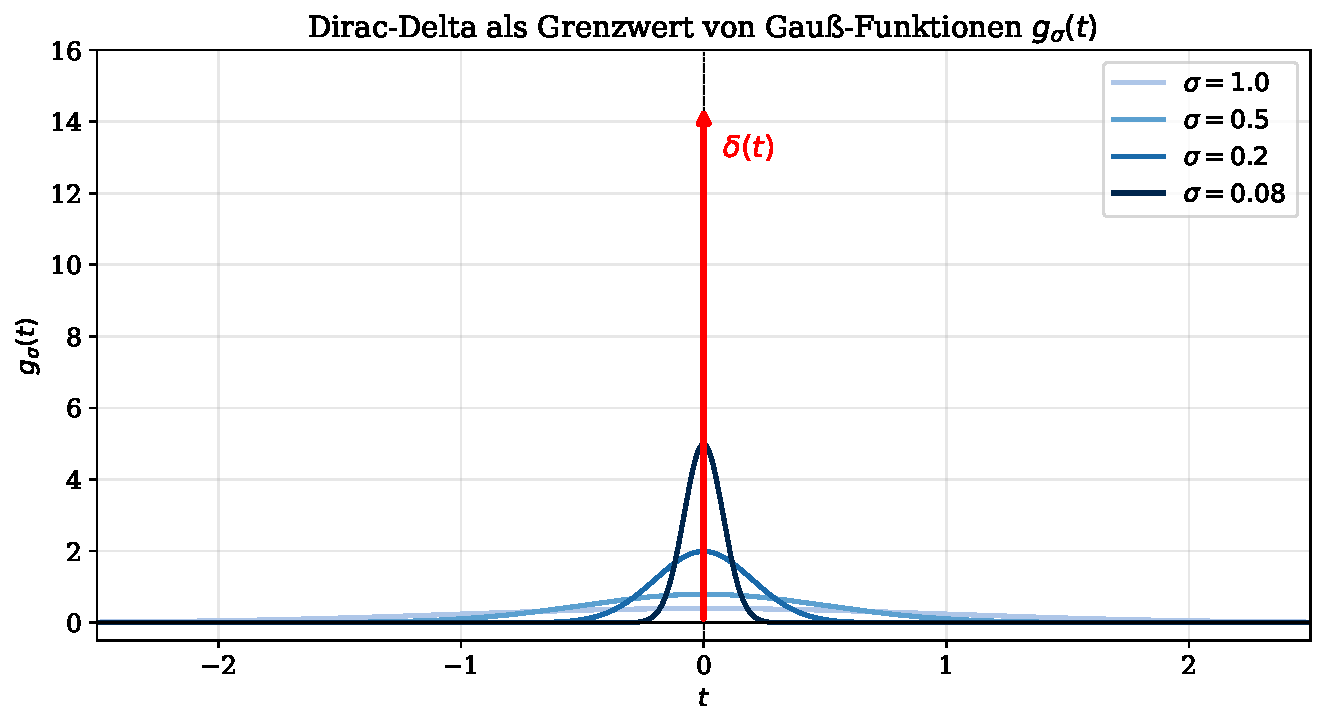
\includegraphics[width=0.9\textwidth]{plot1_gauss_grenzwert.pdf}
\caption{Der Dirac-Impuls als Grenzwert der Gau{\ss}schen N\"aherungsfolge
$g_\varepsilon(t) = \frac{1}{\varepsilon\sqrt{2\pi}}\exp(-t^2/(2\varepsilon^2))$.
Mit kleiner werdendem $\varepsilon$ wird die Spitze bei $t=0$ beliebig hoch,
w\"ahrend die Fl\"ache stets gleich $1$ bleibt. Der rote Pfeil symbolisiert
den Grenzwert $\delta(t)$ im Distributionensinne.}
\label{fig:gauss}
\end{figure}

\begin{bemerkung}
Abbildung~\ref{fig:gauss} illustriert, dass die ``unendliche H\"ohe'' kein Problem ist:
Da simultan die Breite gegen $0$ schrumpft, bleibt das Produkt -- die Fl\"ache -- gleich $1$.
Physikalisch bedeutet dies: Ein immer k\"urzerer, immer st\"arkerer Impuls gleicher Energie.
\end{bemerkung}

% =====================================================================
\section{Eigenschaften des Dirac-Impulses}
\label{sec:eigenschaften}
% =====================================================================

\subsection{Siebungseigenschaft}

Die Siebungseigenschaft ist die wichtigste praktische Eigenschaft des Dirac-Impulses.

\begin{satz}[Siebungseigenschaft]
\label{satz:siebung}
F\"ur jede stetige Funktion $f: \mathbb{R} \to \mathbb{R}$ und $t_0 \in \mathbb{R}$ gilt:
\[
\int_{-\infty}^{\infty} f(t)\,\delta(t - t_0)\,dt = f(t_0).
\]
\end{satz}

\begin{proof}
Per Definition~\ref{def:dirac} des verschobenen Dirac-Impulses:
\[
\delta(t - t_0)[\varphi] = \varphi(t_0).
\]
F\"ur $\varphi = f$ ergibt sich unmittelbar:
\[
\int_{-\infty}^{\infty} f(t)\,\delta(t - t_0)\,dt
:= \delta(t - t_0)[f] = f(t_0).
\]

\textbf{Alternativbeweis \"uber Grenzwertfolge:} Sei $g_\varepsilon$ die Gau{\ss}sche Folge. Dann:
\begin{align*}
\lim_{\varepsilon \to 0} \int_{-\infty}^{\infty} f(t)\,g_\varepsilon(t - t_0)\,dt
&= \lim_{\varepsilon \to 0} \int_{-\infty}^{\infty} f(t)
   \cdot \frac{1}{\varepsilon\sqrt{2\pi}}e^{-(t-t_0)^2/(2\varepsilon^2)}\,dt \\
&\stackrel{u=(t-t_0)/\varepsilon}{=}
   \lim_{\varepsilon \to 0} \frac{1}{\sqrt{2\pi}}
   \int_{-\infty}^{\infty} f(t_0 + \varepsilon u)\,e^{-u^2/2}\,du.
\end{align*}
Da $f$ stetig und die Gau{\ss}glocke $e^{-u^2/2}$ integrierbar ist, erlaubt der
Satz \"uber dominierte Konvergenz das Vertauschen von Grenzwert und Integral:
\[
= \frac{1}{\sqrt{2\pi}} \int_{-\infty}^{\infty} f(t_0)\,e^{-u^2/2}\,du
= f(t_0) \cdot \frac{1}{\sqrt{2\pi}} \cdot \sqrt{2\pi} = f(t_0). \qquad \qedhere
\]
\end{proof}

\begin{figure}[H]
\centering
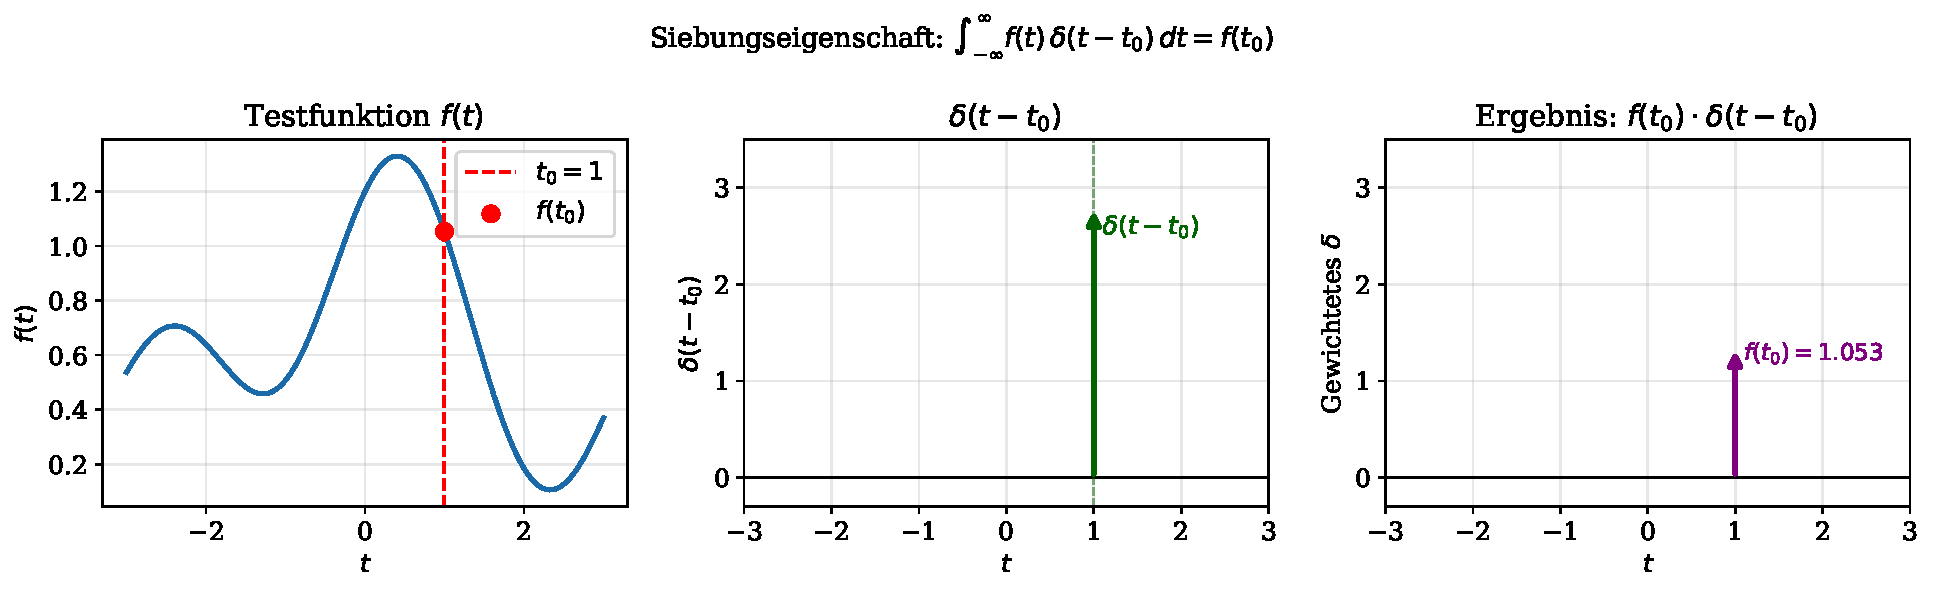
\includegraphics[width=\textwidth]{plot2_siebung.pdf}
\caption{Illustration der Siebungseigenschaft. Links: die Testfunktion $f(t)$.
Mitte: der verschobene Dirac-Impuls $\delta(t - t_0)$ bei $t_0 = 1$.
Rechts: Das Produkt $f(t)\cdot\delta(t-t_0)$ liefert nach Integration genau den Funktionswert $f(t_0)$.}
\label{fig:siebung}
\end{figure}

\subsection{Symmetrie (gerade Distribution)}

\begin{satz}[Symmetrie]
\label{satz:symmetrie}
Der Dirac-Impuls ist eine \emph{gerade} Distribution:
\[
\delta(-t) = \delta(t).
\]
\end{satz}

\begin{proof}
Wir werten $\delta(-t)$ an einer Testfunktion $\varphi$ aus. \"Anderung der Integrationsvariable
$s = -t$, $ds = -dt$:
\[
\delta(-t)[\varphi] := \int_{-\infty}^{\infty} \delta(-t)\,\varphi(t)\,dt
= \int_{\infty}^{-\infty} \delta(s)\,\varphi(-s)\,(-ds)
= \int_{-\infty}^{\infty} \delta(s)\,\varphi(-s)\,ds
= \varphi(0).
\]
Andererseits: $\delta(t)[\varphi] = \varphi(0)$.
Da beide Ausdr\"ucke f\"ur alle $\varphi$ gleich sind, folgt $\delta(-t) = \delta(t)$.
\end{proof}

\subsection{Skalierungseigenschaft}

\begin{satz}[Skalierungseigenschaft]
\label{satz:skalierung}
F\"ur $a \in \mathbb{R} \setminus \{0\}$ gilt:
\[
\delta(a\,t) = \frac{1}{|a|}\,\delta(t).
\]
\end{satz}

\begin{proof}
Sei $\varphi \in \mathcal{D}(\mathbb{R})$ beliebig. Wir berechnen $\delta(at)[\varphi]$.

\textbf{Fall 1: $a > 0$.}
Substitution $s = at$, $ds = a\,dt$, $dt = ds/a$:
\[
\int_{-\infty}^{\infty} \delta(at)\,\varphi(t)\,dt
= \int_{-\infty}^{\infty} \delta(s)\,\varphi\!\left(\frac{s}{a}\right)\frac{ds}{a}
= \frac{1}{a}\,\varphi\!\left(\frac{0}{a}\right) = \frac{1}{a}\,\varphi(0).
\]

\textbf{Fall 2: $a < 0$.}
Substitution $s = at$, $ds = a\,dt < 0$, Integrationsgrenzen tauschen:
\[
\int_{-\infty}^{\infty} \delta(at)\,\varphi(t)\,dt
= \int_{\infty}^{-\infty} \delta(s)\,\varphi\!\left(\frac{s}{a}\right)\frac{ds}{a}
= -\frac{1}{a}\,\varphi(0) = \frac{1}{|a|}\,\varphi(0).
\]

In beiden F\"allen gilt $\delta(at)[\varphi] = \frac{1}{|a|}\,\varphi(0) = \frac{1}{|a|}\,\delta(t)[\varphi]$.
Da $\varphi$ beliebig, folgt $\delta(at) = \frac{1}{|a|}\delta(t)$.
\end{proof}

\begin{korollar}
F\"ur $a = -1$ ergibt sich der Symmetriesatz~\ref{satz:symmetrie} als Spezialfall:
$\delta(-t) = \frac{1}{|-1|}\delta(t) = \delta(t)$.
\end{korollar}

\subsection{Ableitung der Heaviside-Funktion}

\begin{definition}[Heaviside-Funktion]
Die \emph{Heaviside-Stufenfunktion} ist definiert durch:
\[
\Theta(t) := \begin{cases} 1 & t > 0 \\ \frac{1}{2} & t = 0 \\ 0 & t < 0. \end{cases}
\]
\end{definition}

\begin{satz}[Zusammenhang mit der Heaviside-Funktion]
\label{satz:heaviside}
Im Sinne der Distributionentheorie gilt:
\[
\frac{d}{dt}\Theta(t) = \delta(t).
\]
\end{satz}

\begin{proof}
Die Ableitung von $\Theta$ im Distributionensinne ist definiert durch
\[
\Theta'[\varphi] := -\Theta[\varphi'] = -\int_{-\infty}^{\infty} \Theta(t)\,\varphi'(t)\,dt.
\]
Wegen $\Theta(t) = 1$ f\"ur $t > 0$ und $\Theta(t) = 0$ f\"ur $t < 0$:
\[
= -\int_{0}^{\infty} \varphi'(t)\,dt = -\Bigl[\varphi(t)\Bigr]_{0}^{\infty}
= -\bigl(\varphi(\infty) - \varphi(0)\bigr).
\]
Da $\varphi$ kompakten Tr\"ager hat, gilt $\varphi(\infty) = 0$:
\[
= -\bigl(0 - \varphi(0)\bigr) = \varphi(0) = \delta[\varphi].
\]
Damit: $\Theta'[\varphi] = \delta[\varphi]$ f\"ur alle $\varphi \in \mathcal{D}$, also $\Theta' = \delta$.
\end{proof}

\begin{figure}[H]
\centering
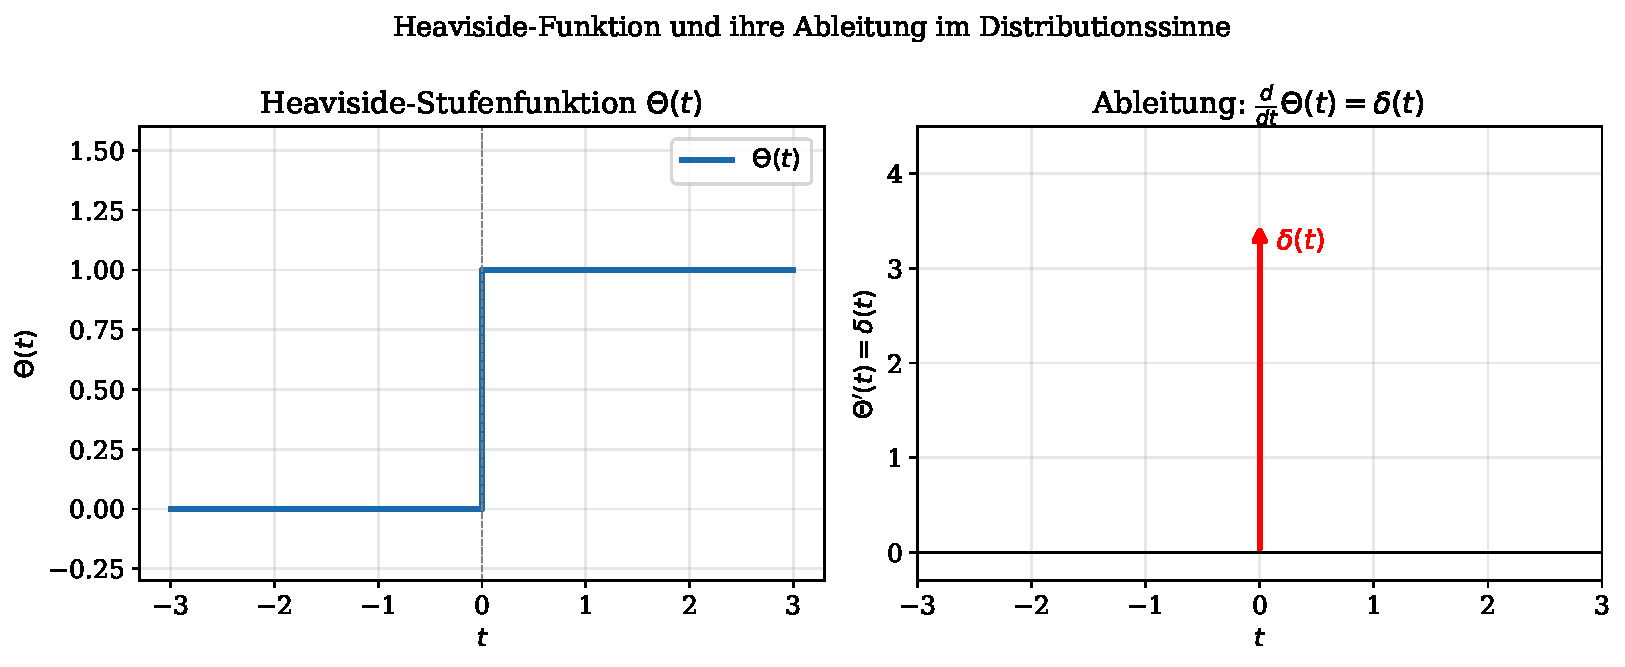
\includegraphics[width=0.9\textwidth]{plot4_heaviside.pdf}
\caption{Links: die Heaviside-Stufenfunktion $\Theta(t)$. Rechts: ihre Ableitung im
Distributionensinne ist der Dirac-Impuls $\delta(t)$. Der vertikale Sprung der
Stufenfunktion um $1$ entspricht formal der unendlichen Konzentration.}
\label{fig:heaviside}
\end{figure}

\subsection{Faltungsidentit\"at}

\begin{satz}[Dirac als Faltungsidentit\"at]
\label{satz:faltung}
F\"ur jede lokal integrierbare Funktion $f$ gilt:
\[
(f * \delta)(t) := \int_{-\infty}^{\infty} f(\tau)\,\delta(t - \tau)\,d\tau = f(t).
\]
Der Dirac-Impuls ist das neutrale Element der Faltungsoperation.
\end{satz}

\begin{proof}
Direkte Anwendung der Siebungseigenschaft (Satz~\ref{satz:siebung}) mit der Substitution
$g(\tau) := \delta(t - \tau)$:
\[
(f * \delta)(t) = \int_{-\infty}^{\infty} f(\tau)\,\delta(t - \tau)\,d\tau = f(t),
\]
wobei die Siebungseigenschaft im zweiten Schritt die Funktion $\tau \mapsto f(\tau)$ an der
Stelle $\tau = t$ auswertet.

Alternativ \"uber die verschobene Version: $\delta(t - \tau) = \delta(\tau - t)$ wegen
Symmetrie. Siebung ergibt dann $f(t)$.
\end{proof}

\subsection{Ableitungen des Dirac-Impulses}

\begin{definition}[Dirac-Ableitungen]
Die $k$-te Ableitung des Dirac-Impulses ist definiert durch:
\[
\delta^{(k)}[\varphi] := (-1)^k\,\varphi^{(k)}(0).
\]
\end{definition}

\begin{satz}[Siebungseigenschaft der Ableitungen]
\label{satz:ableitungen}
F\"ur eine $(k)$-mal stetig differenzierbare Funktion $f$ gilt:
\[
\int_{-\infty}^{\infty} f(t)\,\delta^{(k)}(t)\,dt = (-1)^k\,f^{(k)}(0).
\]
\end{satz}

\begin{proof}
Es gilt nach Definition und $k$-facher partieller Integration (alle Randterme verschwinden,
da $\varphi$ kompakten Tr\"ager hat):
\[
\delta^{(k)}[\varphi] = (-1)^k\,\delta[\varphi^{(k)}] = (-1)^k\,\varphi^{(k)}(0). \qedhere
\]
\end{proof}

% =====================================================================
\section{Fourier-Analyse des Dirac-Impulses}
\label{sec:fourier}
% =====================================================================

\subsection{Fourier-Transformierte}

\begin{satz}[Fourier-Transformierte des Dirac-Impulses]
\label{satz:fourier}
Die Fourier-Transformierte des Dirac-Impulses ist die konstante Funktion $1$:
\[
\mathcal{F}\{\delta(t)\}(\omega) := \int_{-\infty}^{\infty} \delta(t)\,e^{-i\omega t}\,dt = 1.
\]
\end{satz}

\begin{proof}
Direkte Anwendung der Siebungseigenschaft (Satz~\ref{satz:siebung}) mit $f(t) = e^{-i\omega t}$
und $t_0 = 0$:
\[
\mathcal{F}\{\delta\}(\omega)
= \int_{-\infty}^{\infty} \delta(t)\,e^{-i\omega t}\,dt
= \left.\,e^{-i\omega t}\right|_{t=0} = e^{0} = 1. \qquad \qedhere
\]
\end{proof}

\begin{korollar}[Inverse Fourier-Transformation]
Aus dem Fourier-Inversionstheorem folgt:
\[
\delta(t) = \frac{1}{2\pi} \int_{-\infty}^{\infty} e^{i\omega t}\,d\omega.
\]
Dieses Integral divergiert im klassischen Sinne, konvergiert aber schwach gegen $\delta(t)$.
\end{korollar}

\begin{proof}
Sei $\hat{f}(\omega) = 1$. Dann gilt formal:
\[
\mathcal{F}^{-1}\{1\}(t) = \frac{1}{2\pi}\int_{-\infty}^{\infty} 1 \cdot e^{i\omega t}\,d\omega.
\]
F\"ur eine Testfunktion $\varphi \in \mathcal{S}(\mathbb{R})$:
\[
\left\langle \mathcal{F}^{-1}\{1\},\, \varphi \right\rangle
= \frac{1}{2\pi}\int \left(\int e^{i\omega t}\,d\omega\right)\varphi(t)\,dt
= \frac{1}{2\pi}\int \hat\varphi(-\omega)\,d\omega
= \frac{1}{2\pi}\,2\pi\,\varphi(0) = \varphi(0) = \delta[\varphi].
\]
(Es wurde der Plancherel-Satz und $\int\hat\varphi(\omega)\,d\omega = 2\pi\,\varphi(0)$
f\"ur $\varphi \in \mathcal{S}$ benutzt.)
\end{proof}

\begin{figure}[H]
\centering

\includegraphics[width=0.9\textwidth]{plot3_fourier.pdf}
\caption{Fourier-Transformierte des Dirac-Impulses: das Betragsspektrum ist konstant $1$
(weißes Rauschen / weißes Spektrum), und die Phase ist identisch $0$. Dies bedeutet,
dass der Dirac-Impuls alle Frequenzen mit gleicher Amplitude enth\"alt.}
\label{fig:fourier}
\end{figure}

\begin{bemerkung}
Das ``flache Spektrum'' des Dirac-Impulses hat weitreichende Konsequenzen:
In der Systemtheorie gilt $\mathcal{F}\{(f * \delta)\} = \hat{f} \cdot 1 = \hat{f}$,
d.\,h.\ ein System reagiert auf $\delta$ mit seiner vollst\"andigen Frequenz\-charakteristik.
\end{bemerkung}

\subsection{Laplace-Transformierte}

\begin{satz}[Laplace-Transformierte des Dirac-Impulses]
\label{satz:laplace}
F\"ur $\mathrm{Re}(s) > 0$ gilt:
\[
\mathcal{L}\{\delta(t)\}(s) := \int_{0}^{\infty} \delta(t)\,e^{-st}\,dt = 1.
\]
\end{satz}

\begin{proof}
Analogon zum Fourier-Beweis: Siebungseigenschaft mit $f(t) = e^{-st}$ und Integration
\"uber $[0, \infty)$:
\[
\mathcal{L}\{\delta\}(s)
= \int_{0}^{\infty} \delta(t)\,e^{-st}\,dt = e^{-s \cdot 0} = 1. \qquad \qedhere
\]
\end{proof}

% =====================================================================
\section{N\"aherungsfolgen f\"ur den Dirac-Impuls}
\label{sec:naherungen}
% =====================================================================

\begin{definition}[Dirac-Folge]
Eine Folge $(d_\varepsilon)_{\varepsilon > 0}$ von messbaren Funktionen hei{\ss}t
\emph{Dirac-Folge} (oder \emph{approximative Einheit}), wenn:
\begin{enumerate}[label=(\alph*)]
    \item $d_\varepsilon(t) \geq 0$ f\"ur alle $t \in \mathbb{R}$.
    \item $\displaystyle\int_{-\infty}^{\infty} d_\varepsilon(t)\,dt = 1$ f\"ur alle $\varepsilon > 0$.
    \item F\"ur alle $\rho > 0$: $\displaystyle\lim_{\varepsilon \to 0}
          \int_{|t| > \rho} d_\varepsilon(t)\,dt = 0$.
\end{enumerate}
\end{definition}

\begin{satz}
Jede Dirac-Folge konvergiert schwach gegen $\delta$:
$d_\varepsilon \xrightarrow{\mathcal{D}'} \delta$ f\"ur $\varepsilon \to 0$.
\end{satz}

\begin{proof}
Sei $\varphi \in \mathcal{D}(\mathbb{R})$ beliebig und $M := \sup|\varphi|$. Dann:
\begin{align*}
\left|\int d_\varepsilon(t)\,\varphi(t)\,dt - \varphi(0)\right|
&= \left|\int d_\varepsilon(t)[\varphi(t)-\varphi(0)]\,dt\right| \\
&\leq \int_{|t|\leq\rho} d_\varepsilon(t)|\varphi(t)-\varphi(0)|\,dt
    + 2M\int_{|t|>\rho} d_\varepsilon(t)\,dt.
\end{align*}
F\"ur gegebenes $\eta > 0$: W\"ahle $\rho$ so, dass $|\varphi(t)-\varphi(0)| < \eta/2$
f\"ur $|t| < \rho$ (Stetigkeit). Dann ist der erste Term $\leq \eta/2$.
Nach Bedingung (iii) w\"ahle $\varepsilon$ so klein, dass der zweite Term $< \eta/2$.
Insgesamt: $|\int d_\varepsilon \varphi - \varphi(0)| < \eta$. \qedhere
\end{proof}

\subsubsection{Gau{\ss}sche N\"aherungsfolge}
\[
g_\varepsilon(t) = \frac{1}{\varepsilon\sqrt{2\pi}}\,e^{-t^2/(2\varepsilon^2)}.
\]
Normierung: $\int g_\varepsilon\,dt = 1$ (klassisches Gau{\ss}-Integral).

\subsubsection{Rechteck-N\"aherungsfolge}
\[
r_\varepsilon(t) = \frac{1}{\varepsilon}\,\mathbf{1}_{[-\varepsilon/2,\,\varepsilon/2]}(t).
\]
Normierung: $\int r_\varepsilon\,dt = \frac{1}{\varepsilon}\cdot\varepsilon = 1$.

\subsubsection{Dreieck-N\"aherungsfolge}
\[
\Lambda_\varepsilon(t) = \frac{1}{\varepsilon}\max\!\left(0,\, 1 - \frac{|t|}{\varepsilon}\right).
\]
Normierung: $\int \Lambda_\varepsilon\,dt = \frac{1}{\varepsilon}\cdot\varepsilon = 1$
(Dreieckfl\"ache mit Basis $2\varepsilon$ und H\"ohe $1/\varepsilon$).

\subsubsection{Sinc$^2$-N\"aherungsfolge}
\[
s_\varepsilon(t) = \frac{1}{\pi\varepsilon}\,\mathrm{sinc}^2\!\left(\frac{t}{\varepsilon}\right),
\quad \mathrm{sinc}(x) := \frac{\sin(\pi x)}{\pi x}.
\]
Normierung: $\int s_\varepsilon\,dt = 1$ (aus Parseval oder direkter Integration).

\begin{figure}[H]
\centering
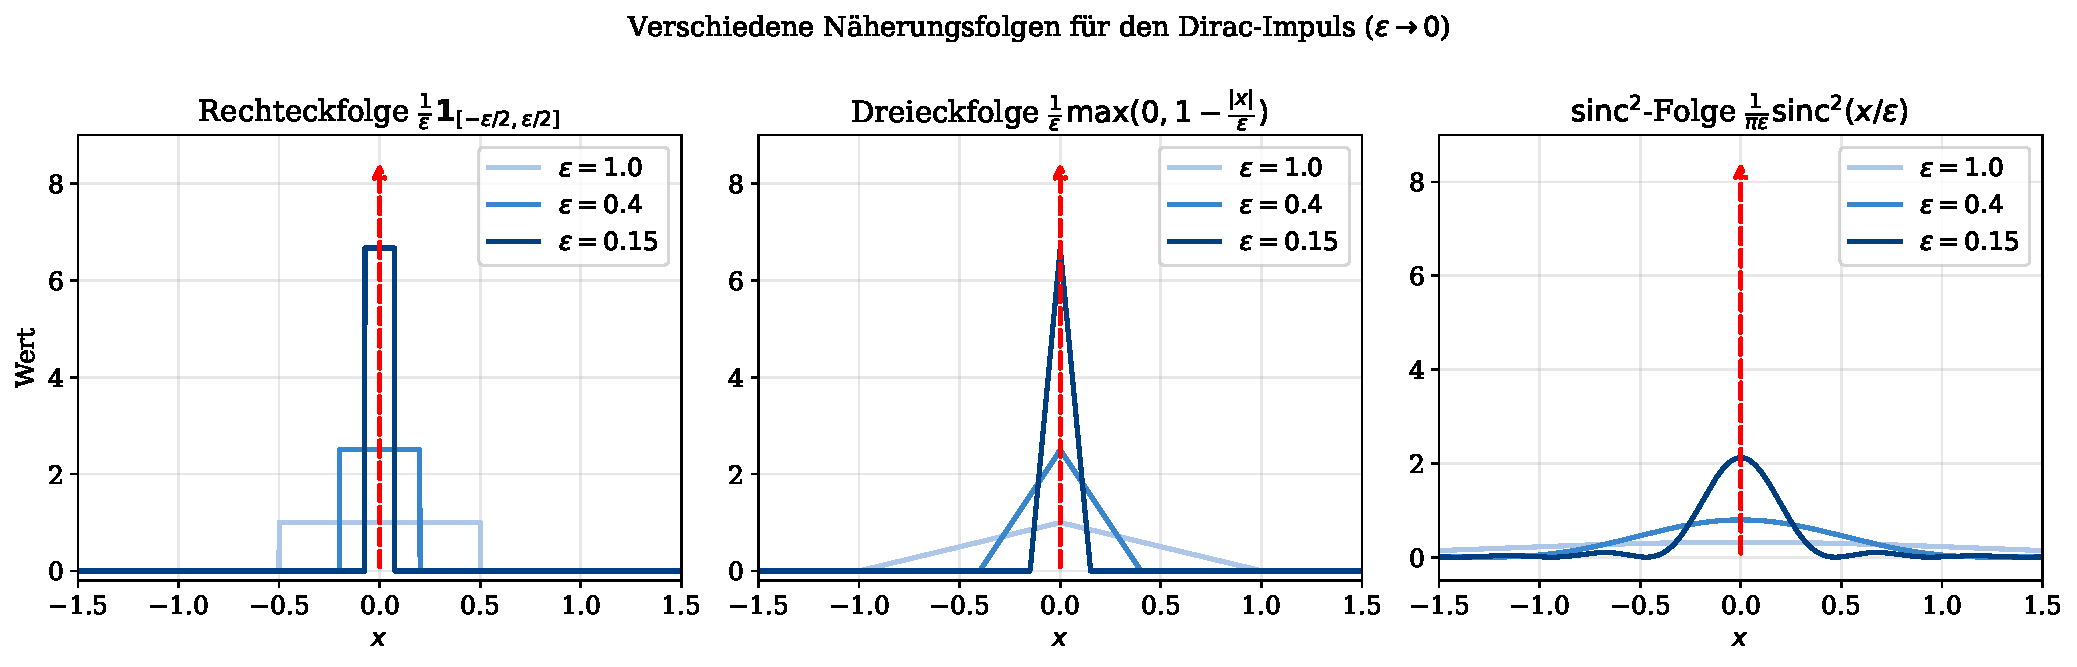
\includegraphics[width=\textwidth]{plot5_approximationen.pdf}
\caption{Drei verschiedene N\"aherungsfolgen f\"ur den Dirac-Impuls bei $\varepsilon \in \{1.0, 0.4, 0.15\}$:
Rechteckfolge (links), Dreieckfolge (Mitte) und Sinc$^2$-Folge (rechts). In allen F\"allen
schrumpft die Breite proportional zu $\varepsilon$, w\"ahrend die H\"ohe um $1/\varepsilon$ w\"achst,
sodass die Fl\"ache konstant $1$ bleibt. Der rote Pfeil symbolisiert den Grenzwert $\delta(t)$.}
\label{fig:approx}
\end{figure}

% =====================================================================
\section{Der Dirac-Kamm und diskrete Abtastung}
\label{sec:kamm}
% =====================================================================

\begin{definition}[Dirac-Kamm / Sha-Funktion]
\label{def:kamm}
Der \emph{Dirac-Kamm} mit Periode $T > 0$ ist definiert als:
\[
\mathrm{III}_T(t) := \sum_{k=-\infty}^{\infty} \delta(t - kT).
\]
\end{definition}

\begin{satz}[Fourier-Reihe des Dirac-Kamms]
\label{satz:kamm_fourier}
Der Dirac-Kamm $\mathrm{III}_T$ ist $T$-periodisch und seine Fourier-Reihe lautet:
\[
\mathrm{III}_T(t) = \frac{1}{T}\sum_{n=-\infty}^{\infty} e^{2\pi i n t/T}.
\]
\end{satz}

\begin{proof}
Da $\mathrm{III}_T$ $T$-periodisch ist, werden die Fourier-Koeffizienten berechnet:
\[
c_n = \frac{1}{T}\int_{-T/2}^{T/2} \mathrm{III}_T(t)\,e^{-2\pi i n t/T}\,dt
= \frac{1}{T}\int_{-T/2}^{T/2} \delta(t)\,e^{-2\pi i n t/T}\,dt
= \frac{1}{T}\,e^{0} = \frac{1}{T}.
\]
(Im Integrationsintervall $[-T/2, T/2]$ tr\"agt nur $k=0$ bei.)
Damit: $\mathrm{III}_T(t) = \sum_n c_n e^{2\pi i n t/T} = \frac{1}{T}\sum_n e^{2\pi i n t / T}$.
\end{proof}

\begin{satz}[Abtastsatz von Shannon-Whittaker]
Sei $f$ bandbegrenzt mit Grenzfrequenz $\omega_c$, d.\,h.\ $\hat{f}(\omega) = 0$ f\"ur
$|\omega| > \omega_c$. Dann wird $f$ durch gleichm\"a{\ss}ige Abtastung mit $T \leq \pi/\omega_c$
vollst\"andig beschrieben:
\[
f(t) = \sum_{k=-\infty}^{\infty} f(kT)\,\mathrm{sinc}\!\left(\frac{t - kT}{T}\right).
\]
\end{satz}

\begin{figure}[H]
\centering
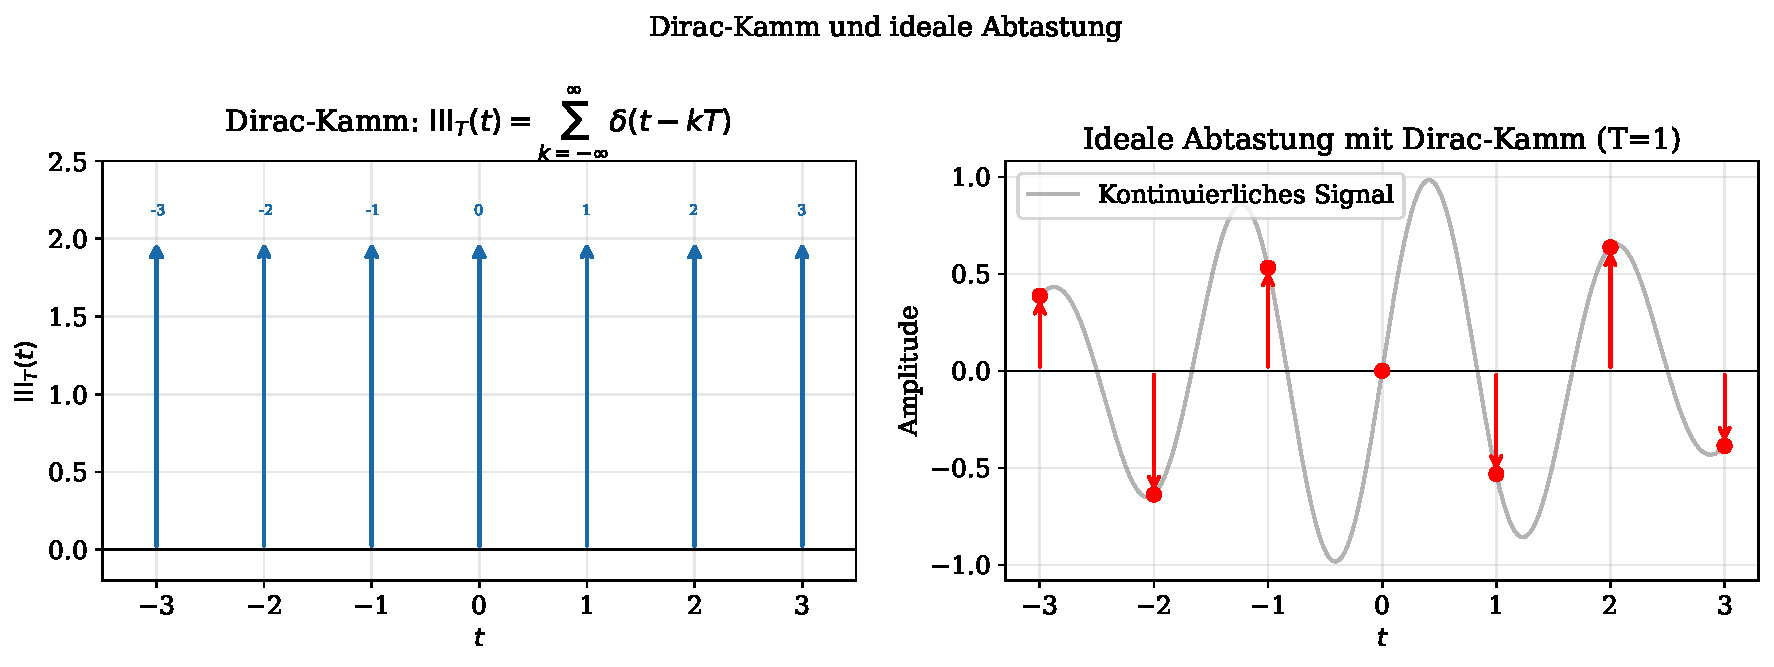
\includegraphics[width=0.9\textwidth]{plot7_dirac_kamm.pdf}
\caption{Links: der Dirac-Kamm $\mathrm{III}_T$ mit $T=1$, eine unendliche Folge
\"aquidistanter Dirac-Impulse. Rechts: ideale Abtastung eines kontinuierlichen Signals
durch Multiplikation mit dem Dirac-Kamm -- die roten Pfeile repr\"asentieren die
Abtastwerte.}
\label{fig:kamm}
\end{figure}

% =====================================================================
\section{Faltung und lineare zeitinvariante Systeme}
\label{sec:lti}
% =====================================================================

\subsection{Impulsantwort eines LTI-Systems}

\begin{definition}[LTI-System]
Ein \emph{lineares zeitinvariantes} (LTI) System ist ein Operator
$\mathcal{H}: L^2(\mathbb{R}) \to L^2(\mathbb{R})$, der f\"ur alle Signale $x$ und
Zeitverschiebungen $\tau$ erf\"ullt:
\begin{itemize}
    \item \textbf{Linearit\"at:} $\mathcal{H}[\alpha x + \beta y] = \alpha\mathcal{H}[x] + \beta\mathcal{H}[y]$.
    \item \textbf{Zeitinvarianz:} Wenn $y(t) = \mathcal{H}[x](t)$, dann $y(t-\tau) = \mathcal{H}[x(\cdot - \tau)](t)$.
\end{itemize}
\end{definition}

\begin{satz}[Impulsantwort charakterisiert LTI-System vollst\"andig]
\label{satz:lti}
Jedes LTI-System wird vollst\"andig durch seine Impulsantwort $h := \mathcal{H}[\delta]$ beschrieben.
F\"ur beliebige Eingabe $x$ gilt:
\[
y(t) = \mathcal{H}[x](t) = (x * h)(t) = \int_{-\infty}^{\infty} x(\tau)\,h(t-\tau)\,d\tau.
\]
\end{satz}

\begin{proof}
Da $\delta$ das neutrale Element der Faltung ist (Satz~\ref{satz:faltung}), l\"asst sich
jedes Signal zerlegen als $x(t) = (x * \delta)(t) = \int x(\tau)\,\delta(t-\tau)\,d\tau$.
Durch Linearit\"at und Zeitinvarianz:
\[
\mathcal{H}[x](t) = \mathcal{H}\!\left[\int x(\tau)\delta(\cdot - \tau)\,d\tau\right](t)
= \int x(\tau)\,\mathcal{H}[\delta(\cdot-\tau)](t)\,d\tau
= \int x(\tau)\,h(t-\tau)\,d\tau.
\]
\end{proof}

\begin{figure}[H]
\centering
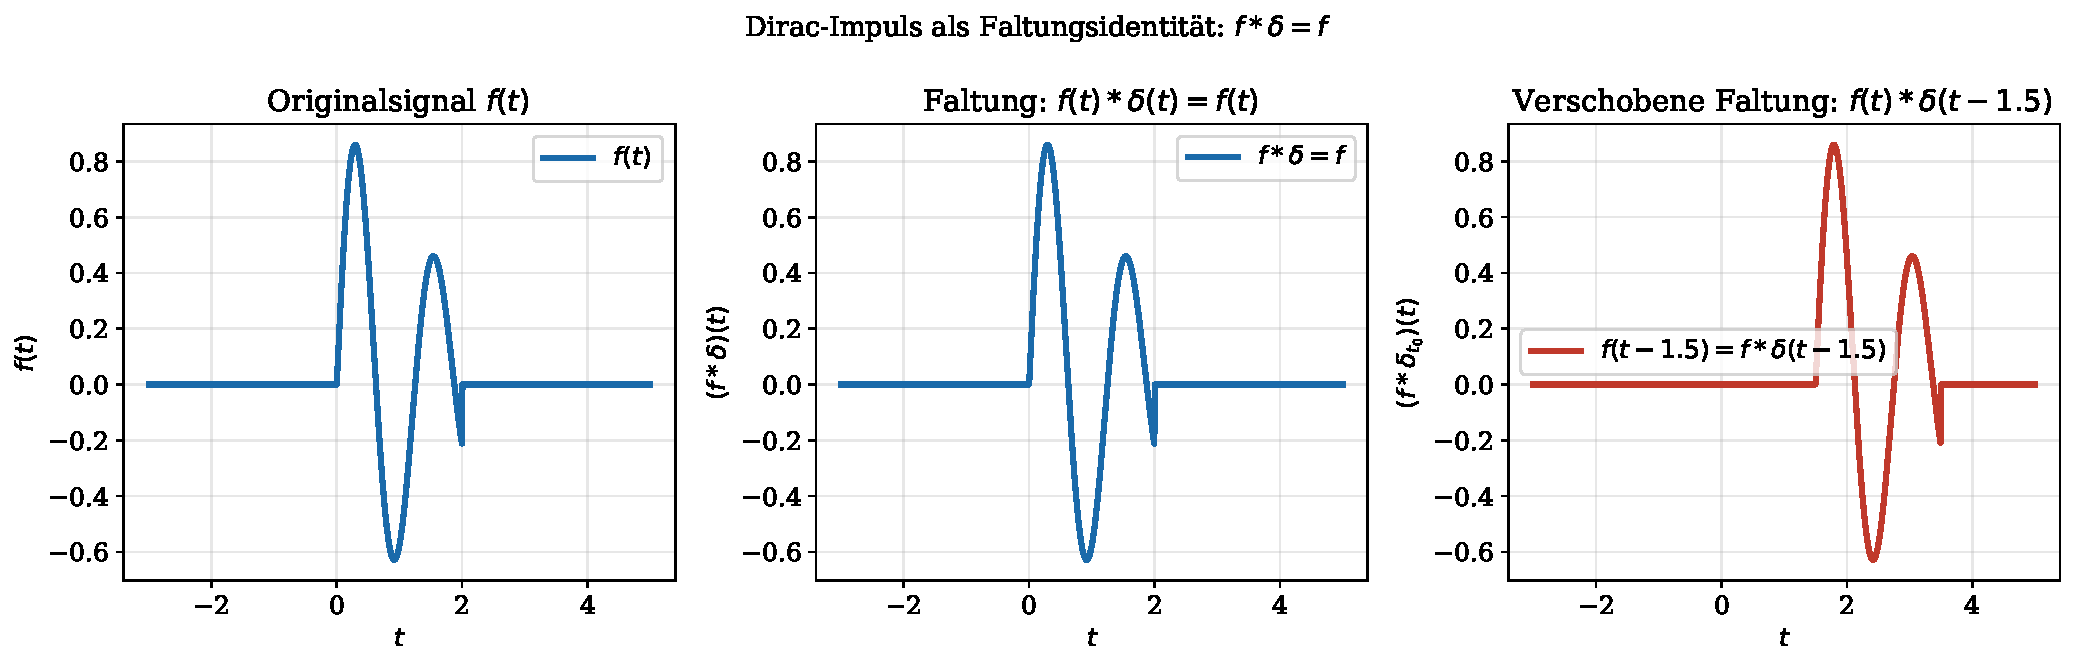
\includegraphics[width=\textwidth]{plot6_faltung.pdf}
\caption{Dirac als neutrales Element der Faltung. Links: Originalsignal $f(t)$.
Mitte: $f * \delta = f$ (keine Ver\"anderung). Rechts: $f * \delta_{t_0}$ verschiebt
das Signal um $t_0 = 1.5$ nach rechts.}
\label{fig:faltung}
\end{figure}

% =====================================================================
\section{Dirac-Impuls in der Quantenmechanik}
\label{sec:quantenmechanik}
% =====================================================================

\subsection{Orthogonalit\"at von Eigenzust\"anden}

In der Quantenmechanik bilden die Ortseigenzust\"ande $|x\rangle$ ein kontinuierliches
Basissystem des Hilbertraums $L^2(\mathbb{R})$.

\begin{satz}[Orthogonalit\"at der Eigenzust\"ande]
F\"ur Ortseigenzust\"ande $|x\rangle$ gilt:
\[
\langle x \mid x' \rangle = \delta(x - x').
\]
\end{satz}

\begin{proof}
Die Vollst\"andigkeitsrelation des kontinuierlichen Spektrums lautet:
\[
\int_{-\infty}^{\infty} |x\rangle\langle x|\,dx = \hat{\mathbf{1}}.
\]
F\"ur einen beliebigen Zustand $|\psi\rangle$:
\[
|\psi\rangle = \hat{\mathbf{1}}|\psi\rangle
= \int |x\rangle\langle x|\psi\rangle\,dx
= \int \psi(x)|x\rangle\,dx.
\]
Andererseits: $\langle x'|\psi\rangle = \psi(x')$ und:
\[
\langle x'|\psi\rangle = \int \psi(x)\,\langle x'|x\rangle\,dx.
\]
Vergleich beider Ausdr\"ucke zeigt, dass $\langle x'|x\rangle$ die Siebungseigenschaft
von $\delta(x-x')$ erf\"ullt. \qedhere
\end{proof}

% =====================================================================
\section{Zusammenfassung der Eigenschaften}
\label{sec:zusammenfassung}
% =====================================================================

\begin{figure}[H]
\centering
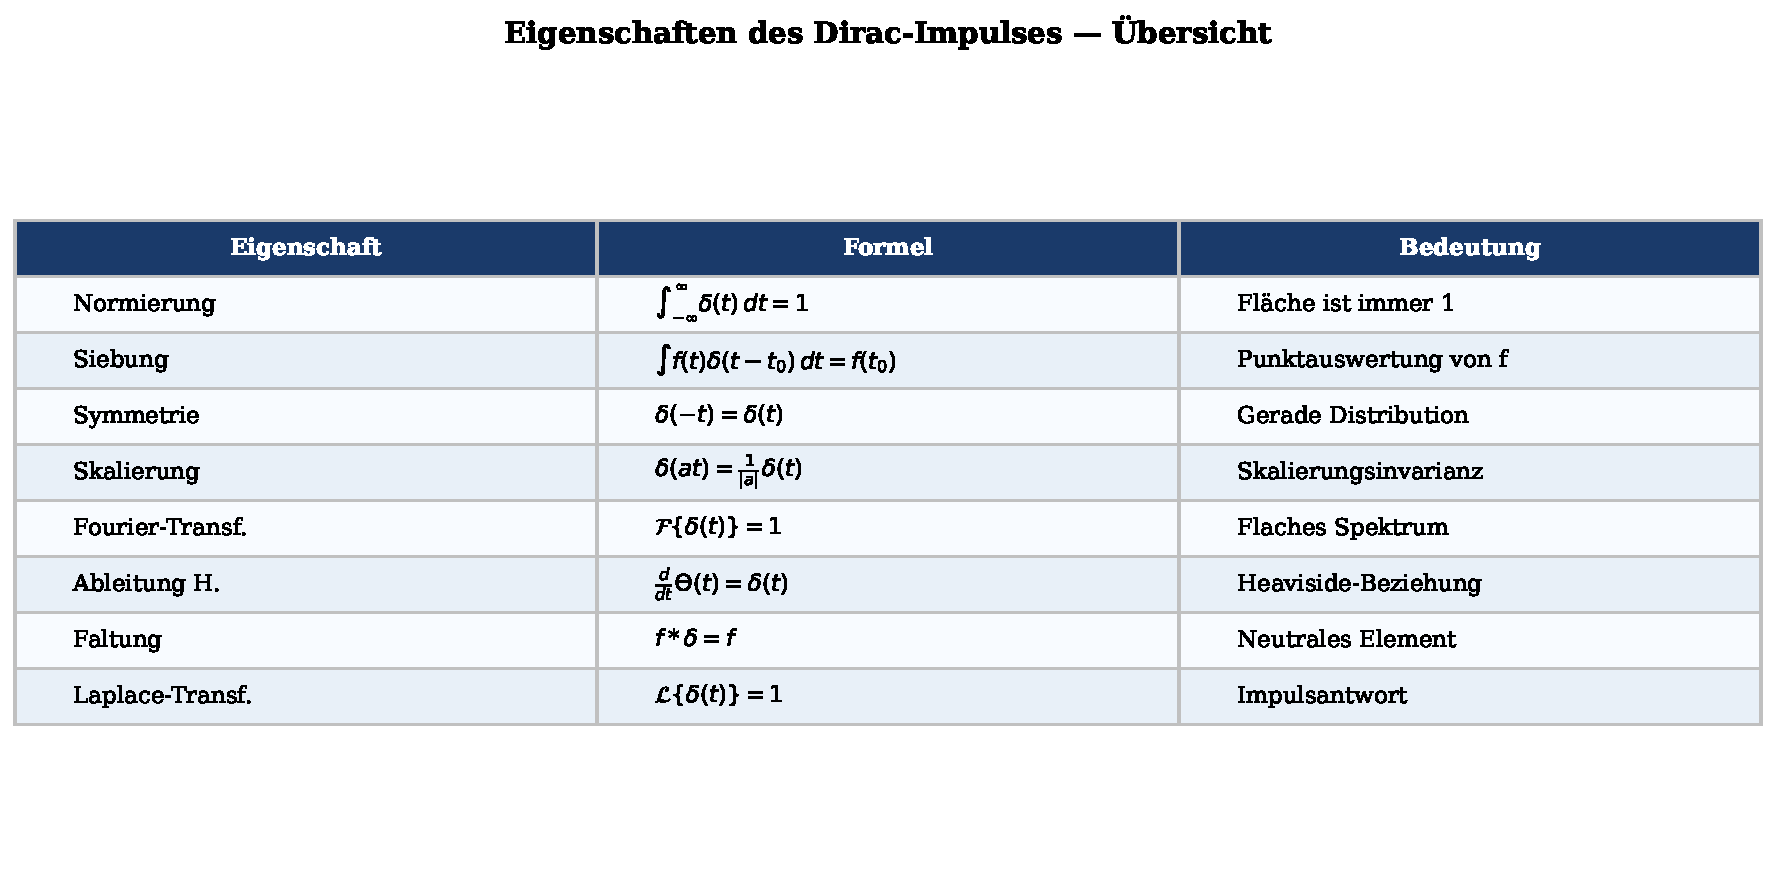
\includegraphics[width=\textwidth]{plot8_eigenschaften_tabelle.pdf}
\caption{\"Ubersicht aller wichtigen Eigenschaften des Dirac-Impulses mit Formeln
und physikalischer Interpretation.}
\label{fig:tabelle}
\end{figure}

Der Dirac-Impuls besitzt folgende formal bewiesene Haupteigenschaften:

\begin{itemize}
    \item \textbf{Normierung:} $\int_{-\infty}^{\infty}\delta(t)\,dt = 1$
          (Satz~\ref{satz:normierung}).
    \item \textbf{Siebung:} $\int f(t)\,\delta(t-t_0)\,dt = f(t_0)$
          (Satz~\ref{satz:siebung}).
    \item \textbf{Symmetrie:} $\delta(-t) = \delta(t)$
          (Satz~\ref{satz:symmetrie}).
    \item \textbf{Skalierung:} $\delta(at) = |a|^{-1}\,\delta(t)$
          (Satz~\ref{satz:skalierung}).
    \item \textbf{Fourier:} $\mathcal{F}\{\delta\}(\omega) = 1$
          (Satz~\ref{satz:fourier}).
    \item \textbf{Laplace:} $\mathcal{L}\{\delta\}(s) = 1$
          (Satz~\ref{satz:laplace}).
    \item \textbf{Heaviside:} $\Theta' = \delta$
          (Satz~\ref{satz:heaviside}).
    \item \textbf{Faltung:} $f * \delta = f$
          (Satz~\ref{satz:faltung}).
    \item \textbf{Ableitungen:} $\int f\,\delta^{(k)}\,dt = (-1)^k f^{(k)}(0)$
          (Satz~\ref{satz:ableitungen}).
    \item \textbf{LTI-Systeme:} Die Impulsantwort $h$ charakterisiert das System vollst\"andig
          (Satz~\ref{satz:lti}).
\end{itemize}

% =====================================================================
\section{Ausblick}
\label{sec:ausblick}
% =====================================================================

Der Dirac-Impuls ist weit mehr als ein technisches Hilfsmittel der Analysis -- er steht
im Zentrum einiger der tiefsten Verbindungen zwischen Mathematik, Physik und Informationstheorie.
In diesem Abschnitt werden vielf\"altige Forschungsrichtungen und offene Fragen skizziert,
die aus der Theorie des Dirac-Impulses erwachsen oder auf ihr aufbauen.

\subsection{Erweiterungen in h\"oheren Dimensionen}

Die $n$-dimensionale Version des Dirac-Impulses ist definiert als:
\[
\delta^{(n)}(\mathbf{x}) := \delta(x_1)\,\delta(x_2)\cdots\delta(x_n),
\quad \mathbf{x} \in \mathbb{R}^n.
\]
In der Quantenfeldtheorie, der Elektrostatik und der Gravitationstheorie spielen diese
Verallgemeinerungen eine zentrale Rolle. Ein offenes Problem besteht darin, Distributions-
theorie auf nicht-kommutativen R\"aumen (z.\,B.\ Moyal-Algebren in der Quantengravitation
\cite{noncommutative_qg}) rigor\"os zu erweitern, da dort die klassische Punktauswertung
des Dirac-Impulses keine direkte Entsprechung hat.

\subsection{Dirac-Impuls und Wavelet-Theorie}

Die Wavelet-Transformation \cite{daubechies1992wavelets} verallgemeinert die Fourier-Analyse
durch lokale, skalierbare Basisfunktionen. Der Dirac-Impuls taucht als Grenzfall auf:
wenn die Analyseskala gegen Null geht, konvergiert das Wavelet gegen eine Dirac-artige
Konzentration. Aktive Forschungsrichtungen umfassen:
\begin{itemize}
    \item \textbf{Sparse-Signal-Rekonstruktion:} Methoden wie Compressed Sensing
          \cite{candes2006compressive} nutzen den Dirac-Impuls als Basisatom f\"ur
          die sparsamste Repr\"asentation von Signalen. Die Frage, unter welchen Bedingungen
          ein Signal durch endlich viele Dirac-Impulse exakt rekonstruiert werden kann,
          ist Gegenstand aktiver Forschung.
    \item \textbf{Super-Resolution:} In der modernen Bildverarbeitung werden Bildmerkmale
          als Summe von Dirac-Impulsen modelliert (``spike-train''), um \"uber die klassische
          Abtastgrenze hinaus aufzul\"osen \cite{candes2014towards}.
    \item \textbf{Neuronale Netze und Sparsit\"at:} Die ReLU-Aktivierungsfunktion,
          Grundlage tiefer neuronaler Netze, hat als Ableitung im Distributionensinne die
          Heaviside-Funktion; deren Ableitung ist wiederum $\delta$. Dieses hierarchische
          Strukturprinzip verbindet Distributionentheorie mit moderner KI-Theorie.
\end{itemize}

\subsection{Dirac-Impuls in der Quantenfeldtheorie}

In der Quantenfeldtheorie (QFT) \cite{peskin1995introduction} sind Felder als
operatorwertige Distributionen zu verstehen -- eine direkte Verallgemeinerung des
Dirac-Impulses auf Feldoperatoren. Die kanonische Vertauschungsrelation
\[
[\hat{\phi}(x), \hat{\pi}(y)] = i\hbar\,\delta^{(3)}(\mathbf{x} - \mathbf{y})
\]
ist das fundamentale Axiom der Quantenfeldtheorie und zeigt, wie der Dirac-Impuls
die Basis des gesamten Geb\"audes bildet. Offene Fragen betreffen insbesondere
die Regularisierung und Renormierung, bei denen Dirac-artige Divergenzen behandelt
werden m\"ussen \cite{zinn-justin2002}.

\subsection{Numerische Approximation und diskrete Signalverarbeitung}

In der diskreten Signalverarbeitung \cite{oppenheim1999discrete} wird der Dirac-Impuls
durch den \emph{Kronecker-Delta} $\delta[n]$ approximiert:
\[
\delta[n] := \begin{cases} 1 & n = 0 \\ 0 & \text{sonst.} \end{cases}
\]
Die Verbindung zwischen dem kontinuierlichen $\delta(t)$ und dem diskreten $\delta[n]$
wird durch den Abtastsatz von Shannon-Whittaker \cite{shannon1949communication} hergestellt.
Aktuelle Herausforderungen umfassen:
\begin{itemize}
    \item \textbf{Sub-Nyquist-Abtastung:} Moderne FRI-Algorithmen (Finite Rate of Innovation,
          \cite{vetterli2002fri}) erlauben die exakte Rekonstruktion von Dirac-Impulsfolgen
          aus weit weniger Abtastwerten als das Nyquist-Theorem vorschreibt.
    \item \textbf{Nicht-gleichm\"a{\ss}ige Abtastung:} Wenn die Abtastzeitpunkte nicht
          \"aquidistant sind, entstehen neue mathematische Herausforderungen, da die
          einfache Faltungsstruktur verloren geht.
    \item \textbf{Quantisierungsfehler:} In realen Systemen f\"uhrt die endliche Aufl\"osung
          des A/D-Wandlers zu einer Verschmierung des Dirac-Impulses; die optimale Quantisierung
          von impulsartigen Signalen ist ein offenes Optimierungsproblem.
\end{itemize}

\subsection{Distributionen auf Mannigfaltigkeiten}

Die Erweiterung der Distributionentheorie auf Riemannsche Mannigfaltigkeiten
\cite{hormander2003analysis} ist ein aktives Forschungsgebiet. Der Dirac-Impuls
$\delta_p$ auf einer Mannigfaltigkeit $M$ ist ein Funktional, das einer Testfunktion
ihren Wert am Punkt $p \in M$ zuordnet:
\[
\delta_p[\varphi] = \varphi(p).
\]
Anwendungen finden sich in:
\begin{itemize}
    \item \textbf{Allgemeiner Relativit\"atstheorie:} Punktquellen der Gravitation
          (Schwarze L\"ocher) werden durch Dirac-Distributionen auf der Raumzeit-Mannigfaltigkeit
          modelliert \cite{geroch1987}.
    \item \textbf{Geometrischer Analysis:} Der Laplace-Beltrami-Operator angewendet auf
          den Dirac-Impuls liefert die Greensche Funktion der Mannigfaltigkeit.
    \item \textbf{Computergeometrie:} In der diskreten geometrischen Verarbeitung werden
          Vertexpunkte von Dreiecksnetzen als Dirac-Impulse auf approximierten Mannigfaltigkeiten
          aufgefasst.
\end{itemize}

\subsection{Dirac-Impuls in der Steuerungstheorie}

In der modernen Regelungstechnik \cite{lunze2014regelungstechnik} und insbesondere
im Kontext von Embedded-Systems-Design \cite{epp2026embedded} bildet die Impulsantwort
eines Systems die Grundlage f\"ur:
\begin{itemize}
    \item \textbf{Systemidentifikation:} Die experimentelle Bestimmung der \"Ubertragungsfunktion
          $H(s) = \mathcal{L}\{h\}(s)$ durch Anregung mit einem impulsnahen Signal.
    \item \textbf{Modellbasierte pr\"adiktive Regelung (MPC):} Impulsantwortmodelle sind
          die Grundlage f\"ur rollende Optimierungshorizonte in MPC-Algoritmen.
    \item \textbf{Kalman-Filter:} Der Voraussageschritt des Kalman-Filters nutzt die
          Systemmatrix $A$, die aus der Impulsantwort gewonnen wird.
    \item \textbf{Echtzeitregelung:} In Echtzeitsystemen (vgl.\ EDF-Scheduling
          \cite{epp2026edf}) muss die Impulsantwortfaltung in deterministischer Zeit
          berechnet werden.
\end{itemize}

\subsection{Nichtlineare Verallgemeinerungen}

Die klassische Distributionentheorie ist auf lineare Strukturen beschr\"ankt: das Produkt
zweier Distributionen ist im Allgemeinen nicht wohldefiniert. Dies ist ein fundamentales
Problem -- insbesondere $\delta^2$ ist keine Distribution.

Aktuelle Forschungsans\"atze zur Behebung dieses Problems:
\begin{itemize}
    \item \textbf{Colombeau-Algebren} \cite{colombeau1984new}: Erweiterung des
          Distributionenraums zu einer assoziativen Algebra, in der Produkte wie
          $\delta^2$ definiert sind, aber die Assoziativit\"at mit der klassischen
          Multiplikation aufgeben.
    \item \textbf{Regularis\-ierung:} Ersetze $\delta$ durch gl\"attende Kerne und
          nehme den Grenzwert nach der Multiplikation -- je nach Reihenfolge k\"onnen
          verschiedene Grenzwerte entstehen (``renormalization ambiguity'').
    \item \textbf{Microlokal-Analysis} \cite{hormander2003analysis}: Beschr\"anke
          die erlaubten Produkte auf Paare von Distributionen, deren Wellenfront-Mengen
          (WF) keine kompatiblen Singularit\"aten aufweisen:
          $\mathrm{WF}(u) + \mathrm{WF}(v) \not\ni 0$.
\end{itemize}

\subsection{Stochastik und Wei{\ss}es Rauschen}

Der Dirac-Impuls ist eng verkn\"upft mit dem Begriff des \emph{wei{\ss}en Rauschens}
\cite{ito1944stochastic}. Das formale Wei{\ss}e-Rauschen-Prozess $W(t)$ ist definiert als
die ``Ableitung'' des Wiener-Prozesses $B(t)$ (Brownsche Bewegung):
\[
W(t) := \frac{dB}{dt}.
\]
Da $B$ nicht differenzierbar ist, muss dies im Distributionensinne verstanden werden.
Die Autokorrelationsfunktion des Wei{\ss}en Rauschens ist:
\[
\mathbb{E}[W(t)W(s)] = \sigma^2\,\delta(t-s),
\]
was unmittelbar die Siebungseigenschaft aufgreift. Forschungsrichtungen umfassen:
\begin{itemize}
    \item Fractional Brownian Motion und verallgemeinerte Dirac-Korrelationen.
    \item Anomale Diffusion mit L\'evy-Prozessen, wo $\delta$ durch $\alpha$-stabile
          Distributionen ersetzt wird.
    \item Stochastische partielle Differentialgleichungen mit Dirac-getriebenem Rauschen.
\end{itemize}

\subsection{Numerische Methoden und Finite-Elemente-Analyse}

Die numerische Behandlung von Punktquellen in partiellen Differentialgleichungen ist
eine algorithmische Herausforderung \cite{brenner2008mathematical}. Das Problem
\[
-\Delta u = \delta_{p}
\]
hat keine herk\"ommliche $H^1$-L\"osung (die Greensche Funktion ist f\"ur $n \geq 2$
singul\"ar). Aktuelle Entwicklungen:
\begin{itemize}
    \item \textbf{Regularisierte FEM:} Ersetze $\delta_p$ durch gl\"attende Gausskerne
          auf der Gitterebene.
    \item \textbf{XFEM (Extended FEM)}: Anreicherung des FEM-Raums mit singul\"aren
          Basisfunktionen, die die Dirac-Singularit\"at korrekt darstellen.
    \item \textbf{Isogeometrische Analysis (IGA):} Nutzung von NURBS-Basisfunktionen,
          die die Singularit\"at glatter approximieren als klassische FEM.
    \item \textbf{Meshfree-Methoden (SPH, RBF):} In der Smoothed Particle Hydrodynamics
          ist jedes Partikel eine Dirac-artige Massenkonzentration.
\end{itemize}

\subsection{Maschinelles Lernen und implizite neuronale Repr\"asentationen}

Ein aktueller Forschungstrend verbindet Distributionentheorie mit modernem Deep Learning:
\begin{itemize}
    \item \textbf{Neural ODEs und Impulssteuerung:} Die Idee, ein System durch eine
          Folge von Dirac-Impulsen zu steuern, f\"uhrt auf diskrete Approximationen von
          Neural ODEs \cite{chen2018neuralode}.
    \item \textbf{Implicit Neural Representations (INR):} Netzwerke wie SIREN
          \cite{sitzmann2020implicit} nutzen sin-Aktivierungen, deren Fourier-Dual
          Dirac-Impulse sind, um hochfrequente Details zu repr\"asentieren.
    \item \textbf{Spike-Kodierung in Spiking Neural Networks (SNN):} In biologisch
          inspirierten SNNs werden Informationen als Zeitpunkte von Dirac-Impulsen
          (Spikes) kodiert -- die gesamte Neuroinformatik basiert letztlich auf dem
          Dirac-Impuls als Kommunikationsatom.
\end{itemize}

\subsection{Offene mathematische Probleme}

Abschlie{\ss}end werden einige unvollst\"andig gel\"oste mathematische Fragen genannt:

\begin{itemize}
    \item \textbf{Dirac-Impuls auf Fraktalen:} Wie ist $\delta$ auf einem Cantor-Menge
          oder einem Sierpinski-Dreieck zu definieren? Selbst\"ahnliche Distributionen
          auf fraktalen Ma{\ss}r\"aumen sind ein junges Forschungsfeld \cite{strichartz1999}.
    \item \textbf{Quantenchaos und Dirac-Spektren:} Die Verteilung der Nullstellen der
          Riemannschen Zeta-Funktion wird durch das GUE-Ensemble der Zufallsmatrizen
          beschrieben; die Dirac-Impulse an diesen Stellen sind Gegenstand der Montgomery-Odlyzko-
          Vermutung und der ungelösten Riemannschen Vermutung.
    \item \textbf{Dirac-Impuls in $p$-adischen R\"aumen:} Die Analysis auf $p$-adischen
          Zahlen f\"uhrt auf eine andere Topologie, in der der Dirac-Impuls andere
          Regularit\"atseigenschaften zeigt \cite{vvz1994}.
\end{itemize}

% =====================================================================
\section*{Danksagung}
% =====================================================================

Der Autor dankt der Universit\"at Bielefeld f\"ur die Bereitstellung von Forschungsressourcen.

% =====================================================================
\begin{thebibliography}{99}

\bibitem{dirac1927}
P.~A.~M. Dirac,
\textit{The Physical Interpretation of the Quantum Dynamics},
Proc.\ Roy.\ Soc.\ London \textbf{A113}, 621--641 (1927).

\bibitem{schwartz1950}
L.~Schwartz,
\textit{Th\'eorie des Distributions},
Hermann, Paris, 1950--1951.

\bibitem{hormander2003analysis}
L.~H\"ormander,
\textit{The Analysis of Linear Partial Differential Operators I},
Springer, Berlin, 4.\ Auflage, 2003.

\bibitem{rudin1991functional}
W.~Rudin,
\textit{Functional Analysis},
McGraw-Hill, New York, 2.\ Auflage, 1991.

\bibitem{daubechies1992wavelets}
I.~Daubechies,
\textit{Ten Lectures on Wavelets},
SIAM, Philadelphia, 1992.

\bibitem{candes2006compressive}
E.~J.\ Cand\`es und T.~Tao,
\textit{Near Optimal Signal Recovery from Random Projections},
IEEE Trans.\ Inf.\ Theory, \textbf{52}(12), 5406--5425, 2006.

\bibitem{candes2014towards}
E.~J.\ Cand\`es und C.~Fernandez-Granda,
\textit{Towards a Mathematical Theory of Super-Resolution},
Comm.\ Pure Appl.\ Math., \textbf{67}(6), 906--956, 2014.

\bibitem{shannon1949communication}
C.~E.\ Shannon,
\textit{Communication in the Presence of Noise},
Proc.\ IRE, \textbf{37}(1), 10--21, 1949.

\bibitem{oppenheim1999discrete}
A.~V.\ Oppenheim, R.~W.\ Schafer,
\textit{Discrete-Time Signal Processing},
Prentice Hall, 3.\ Auflage, 1999.

\bibitem{vetterli2002fri}
M.~Vetterli, P.~Marziliano, T.~Blu,
\textit{Sampling Signals with Finite Rate of Innovation},
IEEE Trans.\ Signal Process., \textbf{50}(6), 1417--1428, 2002.

\bibitem{peskin1995introduction}
M.~E.\ Peskin, D.~V.\ Schroeder,
\textit{An Introduction to Quantum Field Theory},
Addison-Wesley, Reading, 1995.

\bibitem{zinn-justin2002}
J.~Zinn-Justin,
\textit{Quantum Field Theory and Critical Phenomena},
Clarendon Press, Oxford, 4.\ Auflage, 2002.

\bibitem{noncommutative_qg}
A.~Connes,
\textit{Noncommutative Geometry},
Academic Press, San Diego, 1994.

\bibitem{colombeau1984new}
J.-F.\ Colombeau,
\textit{New Generalized Functions and Multiplication of Distributions},
North-Holland, Amsterdam, 1984.

\bibitem{geroch1987}
R.~Geroch,
\textit{Mathematical Physics},
University of Chicago Press, Chicago, 1985.

\bibitem{ito1944stochastic}
K.~It\^o,
\textit{Stochastic Integral},
Proc.\ Imp.\ Acad.\ Tokyo, \textbf{20}(8), 519--524, 1944.

\bibitem{brenner2008mathematical}
S.~C.\ Brenner, L.~R.\ Scott,
\textit{The Mathematical Theory of Finite Element Methods},
Springer, New York, 3.\ Auflage, 2008.

\bibitem{chen2018neuralode}
R.~T.~Q.\ Chen, Y.~Rubanova, J.~Bettencourt, D.~Duvenaud,
\textit{Neural Ordinary Differential Equations},
NeurIPS 2018, arXiv:1806.07366.

\bibitem{sitzmann2020implicit}
V.~Sitzmann, J.~Martel, A.~Bergman, D.~Lindell, G.~Wetzstein,
\textit{Implicit Neural Representations with Periodic Activation Functions},
NeurIPS 2020, arXiv:2006.09661.

\bibitem{strichartz1999}
R.~S.\ Strichartz,
\textit{Analysis on Fractals},
Notices Amer.\ Math.\ Soc., \textbf{46}(10), 1199--1208, 1999.

\bibitem{vvz1994}
V.~S.\ Vladimirov, I.~V.\ Volovich, E.~I.\ Zelenov,
\textit{$p$-adic Analysis and Mathematical Physics},
World Scientific, Singapore, 1994.

\bibitem{lunze2014regelungstechnik}
J.~Lunze,
\textit{Regelungstechnik 1},
Springer Vieweg, 10.\ Auflage, 2014.

\bibitem{epp2026embedded}
S.~Epp,
\textit{Optimierung des Embedded-Systems-Design durch den Subgraph-Algorithmus},
Universit\"at Bielefeld, 2026.

\bibitem{epp2026edf}
S.~Epp,
\textit{EDF+ Real-Time Scheduling Algorithm},
Universit\"at Bielefeld, 2026.

\end{thebibliography}

\end{document}
